\subsubsection{Project $\pi$}

\url{https://en.wikipedia.org/wiki/Projection_(relational_algebra)}\\

\begin{figure}[h]
	\centering
	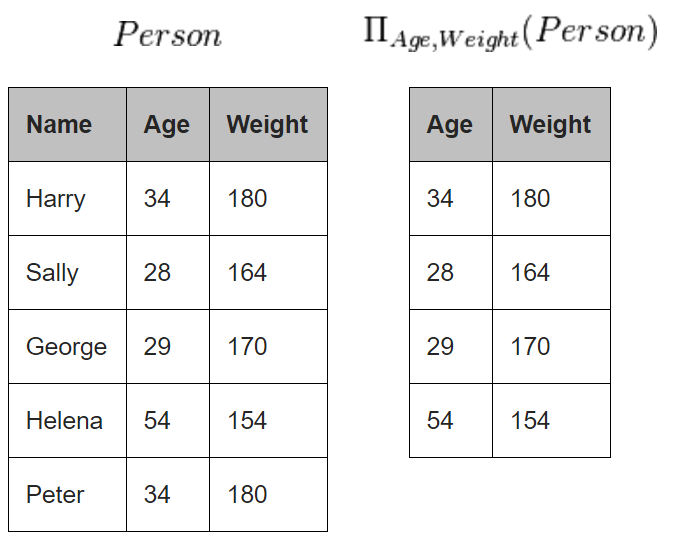
\includegraphics[width=0.6\linewidth]{figs/spm6/project}
	\caption{RA og project}
	\label{fig:project}
\end{figure}


Denne operator bruges til at lave en \textit{vertical partitionering} og giver os kun de kolonner som vi er interesserede i. 
%Eksempelvis, hvis vi kun er interessede i navn og email for alle i tabellen på side~\pageref{tab:stud}, kan vi skrive følgende med RA:
%
%\begin{equation}
%\pi_{navn, email}(Studerende)
%\end{equation}
%
%Hvilket så vil give os følgende tabel:
%
%\begin{table}[H]
%	\centering
%	\begin{tabular}{ll}
%		\toprule
%		\textbf{Navn}	& \textbf{Email}	\\
%		\midrule
%		John Derp		& john@derp.me		\\			
%		Hans Hansen		& hans@landmand.dk	\\			
%		Brian Jensen	& brian@randers.dk	\\			
%		Signe Andersen	& signe@hotmail.com	\\
%		\bottomrule
%	\end{tabular}
%	\caption{Studerende med navn og email.}
%\end{table}